\subsection{The Short-Baseline Neutrino Program}
\label{sec:sbn_program}
In 2014, the Particle Physics Projects Prioritization Panel (P5) recommended a near-term, world-leading, short-baseline experimental neutrino program with strong international and domestic participation. Specifically \cite{Ritz2014}:

\begin{itemize}
    \item \textbf{P5 Recommendation \#12:} In collaboration with international partners, develop a coherent short- and long-baseline neutrino program hosted at Fermilab.
    \item \textbf{P5 Recommendation \#15:} Select and perform in the short term a set of small-scale short-baseline experiments that can conclusively address experimental hints of physics beyond the three-neutrino paradigm. Some of these experiments should use liquid argon to advance the technology and build the international community for LBNF at Fermilab.
\end{itemize}

In the modern day, the Long-Baseline Neutrino Facility (LBNF) is the infrastructure project at Fermilab which will host the Deep Underground Neutrino Experiment (DUNE). These recommendations are the genesis of the SBN Program at Fermilab, as proposed in \cite{Acciarri2015}, which is dedicated to resolving the short-baseline neutrino anomalies observed in the LSND and MiniBooNE experiments while furthering the development of the LArTPC technology for DUNE.

\subsubsection{Physics Goals of the SBN Program}
\label{sec:sbn_physics}

The Short-Baseline Neutrino (SBN) Program brings together three detectors utilizing the LArTPC technology and located on-axis in the Booster Neutrino Beam. Figure \ref{fig:sbn_program_diagram} schematically summarizes the locations of the three detectors relative to the BNB target and their sizes. The detector locations were chosen to optimize the sensitivity to neutrino oscillations and to minimize the impact of flux systematic uncertainties. SBND is located closest to the BNB target and is designed to characterize the neutrino flux. The two far detectors, MicroBooNE and ICARUS, are positioned to have complementary sensitivities to short-baseline neutrino oscillations. The shared technology and beamline of the three detectors means that common systematic uncertainties cancel in the comparison of the results from the three detectors to first order. As an example, if the neutrino flux or $\nu$-Ar cross sections are mis-modeled, the effect will be the same in all three detectors, and the comparison of the results from the three detectors will be unaffected. This is a significant advantage of the SBN Program over previous experiments which have observed short-baseline neutrino anomalies.

\begin{figure}
    \centering
    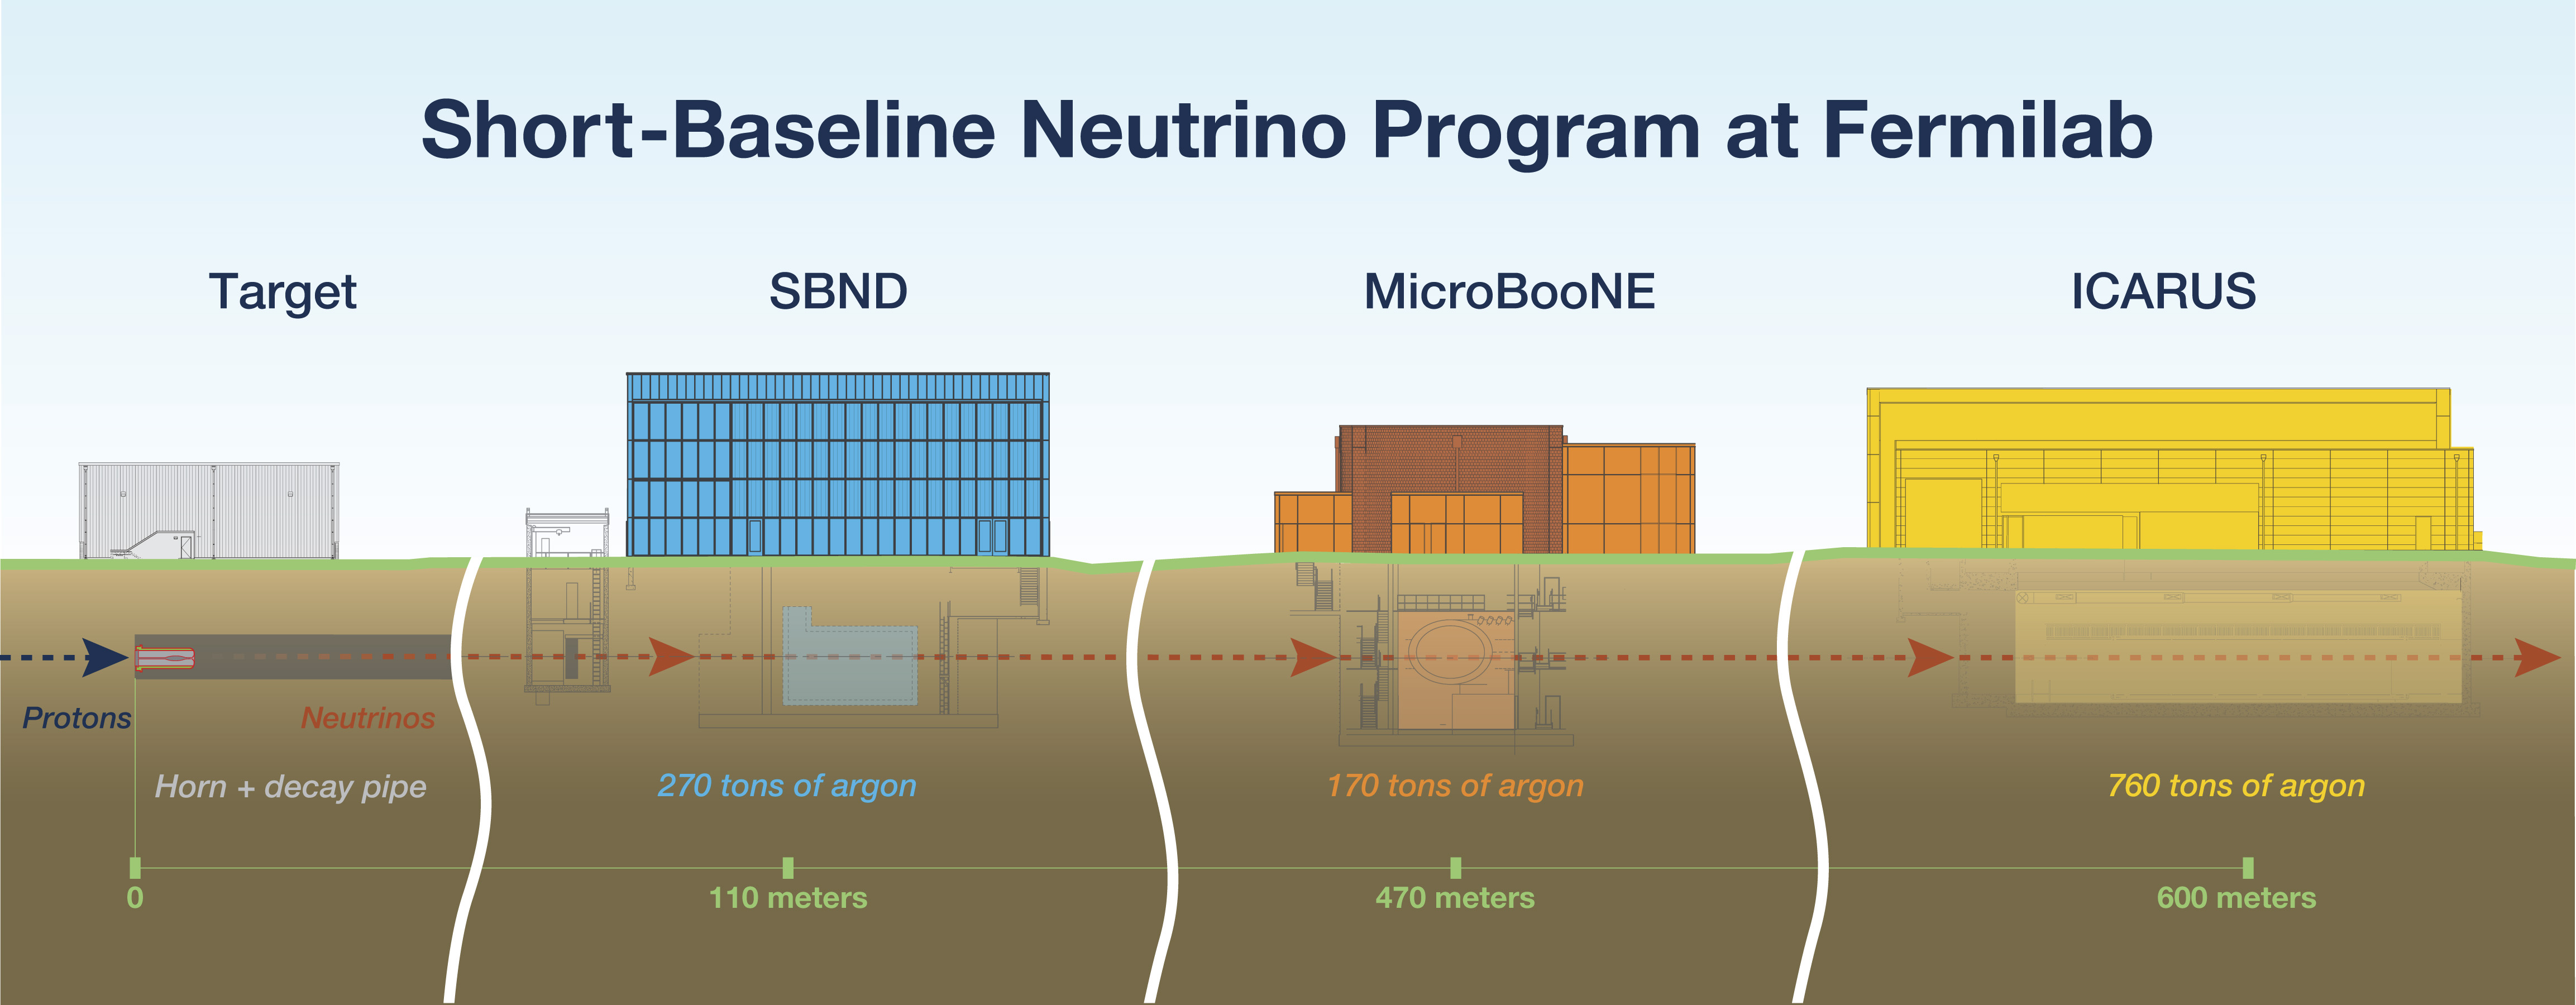
\includegraphics[width=\textwidth]{figures/introduction/sbn_program_diagram.jpg}
    \caption{Schematic diagram of the Short-Baseline Neutrino Program at Fermilab. The three detectors, SBND, MicroBooNE, and ICARUS T600, are located on-axis in the Booster Neutrino Beam. Image from Fermilab Visual Media Services.}
    \label{fig:sbn_program_diagram}
\end{figure}

The SBN Program, following the recommendations of P5, has four primary physics goals:

\begin{itemize}
    \item Conclusively resolve anomalies observed at short-baselines
    \item Characterize $\nu-Ar$ interactions
    \item Search for physics beyond the Standard Model
    \item Develop the LArTPC technology, software, and analysis tools for DUNE
\end{itemize}

\noindent
These four primary physics goals will each be described in detail below.

\paragraph*{Conclusively resolve anomalies observed at short-baselines}
The primary physics goal of the SBN Program is to conclusively resolve the short-baseline neutrino anomalies observed in the LSND and MiniBooNE experiments. The 3+1 minimal extension to the three-neutrino model provides effective oscillation probabilities for $\nu_\mu$ disappearance and $\nu_e$ appearance with which the SBN Program can explore the parameter space of the sterile neutrino hypothesis:

\begin{equation}
    \begin{aligned}
        P_{\nu_\mu \rightarrow \nu_\mu}^{3+1} & = 1 - 4 \left| U_{\mu 4} \right|^2 \left( 1 - \left| U_{\mu 4} \right|^2 \right) \sin^2{\frac{\Delta m_{41}^2L}{4E}}\\
        & \equiv 1 - \sin^2{2\theta_{\mu\mu}} \sin^2{\frac{\Delta m_{41}^2L}{4E}}
    \end{aligned}
    \label{eq:sbn_sterile_oscillation_probability_numu_disappearance}
\end{equation}

\begin{equation}
    \begin{aligned}
        P_{\nu_\mu \rightarrow \nu_e}^{3+1} & = 4 \left| U_{\mu 4} \right|^2 \left| U_{e 4} \right|^2 \sin^2{\frac{\Delta m_{41}^2L}{4E}}\\
        & \equiv \sin^2{2\theta_{\mu e}} \sin^2{\frac{\Delta m_{41}^2L}{4E}}
    \end{aligned}
    \label{eq:sbn_sterile_oscillation_probability_nue_appearance}
\end{equation}

\noindent
These two channels are the primary targets with the highest sensitivity due to the fact that the BNB is a predominately $\nu_\mu$ beam.

Electron neutrino candidates include intrinsic $\nu_e$ CC interactions as well as other beam-related mis-identified backgrounds. The SBN proposal \cite{Acciarri2015} chose a signal definition which requires the presence of a single electron shower with $E_e >$ 200 MeV and with an assumed identification efficiency of 80\% after restricting the candidate interaction vertices to the fiducial volume. The fiducial volume cut requires that the vertex of the interaction to be at least \qty[mode=text]{25}{cm} from the faces parallel to the beam, \qty[mode=text]{30}{cm} from the detector face upstream of the beam, and \qty[mode=text]{50}{cm} from the detector face downstream of the beam in order to maintain reconstruction fidelity. The 80\% efficiency target was estimated from hand-scanning simulated events and requires verification with automated reconstruction algorithms. 

In addition to the intrinsic $\nu_e$ CC interactions, there are several sources of background which can mimic the signal. Neutrinos interacting through NC channels may produce $\gamma$ showers above the 200 MeV shower cut, which can be mis-identified as electrons. For example, NC interactions which produce any number of $\pi^0$ in the final state or radiative resonant decays are sources of $\gamma$'s which can mimic the signal. Cuts on the number of reconstructed showers in an interaction along with conversion gap and $dE/dx$ cuts, which leverage the excellent spatial resolution and calorimetry of the LArTPC technology, can be used to suppress these backgrounds. 

Due to the relatively plentiful $\nu_\mu$ CC interactions, mis-reconstructed $\nu_\mu$ CC interactions with an electromagnetic shower can also fake a $\nu_e$ CC interaction. If the muon is not reconstructed or if the muon is mis-identified as a pion, the interaction may meet the signal definition. Tracks that are sufficiently long are almost entirely muons, so a cut on the track length can be used to suppress these backgrounds. Cosmogenic photons, either from a cosmic muon or produced in the atmospheric shower itself, may also create electromagnetic showers which can mimic the signal. Additional shielding in the form of a concrete overburden can reduce the rate of primary photons significantly, but does not eliminate the background imposed by primary cosmic muons. Instead, reconstruction cuts utilizing the interaction topology and timing information can be used to suppress these backgrounds, or robust estimation of the cosmic background through simulation or data can be used to characterize the background.

$\nu_\mu$ CC candidates are similarly selected assuming an 80\% reconstruction and identification efficiency after a fiducial volume cut has been applied (the same as described previously). This signal definition requires a muon in the interaction's final state. Beam-related backgrounds include NC charged pion production, as charged pions have a similar $dE/dx$ profile to muons and may therefore be mis-identified as muons. Charged pion tracks are typically quite short with most traveling less than half a meter in liquid argon, so a cut on the track length can be used to suppress these backgrounds. A minimum length of 50 cm for the candidate muon track was chosen in the SBN proposal to minimize these backgrounds.

Cosmogenic muons are a significant background for the $\nu_\mu$ disappearance search. Cosmogenic muons are most often out-of-time with respect to the beam window, so a cut on the timing of the interaction can be used as a first step to suppress these backgrounds. Furthermore, muons entering the detector can be tagged in a variety of ways. A muon which stops in the detector will have one end point at the detector boundary and exhibit a clear stopping signature in the form of a high rate of charge deposition at the opposite end of the track. The cosmic ray tagging system, which is a subsystem surrounding each of the three SBN detectors dedicated to tagging particles as they enter or exit the detector, can also be used to provide further cosmic background rejection. The combination of interaction timing and the requirement of an exiting or fully-contained track topology are sufficient to suppress the cosmic background to a manageable level.

Precise measurement of the energy of the neutrino interaction is essential for optimal sensitivity to neutrino oscillations and is contingent upon the calorimetric capabilities of the LArTPC technology. The reconstruction of the electron neutrino energy relies on the precise reconstruction of the resulting electromagnetic shower's energy. This is done by summing the charge deposited in the shower and converting it to an energy by accounting for the electronics gain, electron lifetime, and recombination effects. 

The reconstruction of the muon neutrino energy is dependant on whether the resulting muon track is fully contained or exiting. If the muon is fully contained, the energy can be estimated using the length of the muon track and the theoretically well-known rate of energy loss for muons in liquid argon. If the muon exits the volume, its energy must instead be estimated using the degree of scattering from Coulomb interactions present along the track. In order to attain sufficient energy resolution through multiple Coulomb scattering measurements, the SBN proposal places a 100 centimeter minimum length cut on exiting muon tracks.

\paragraph*{Characterize $\nu-\mathrm{Ar}$ interactions}
Precise neutrino-nucleus cross section measurements are a fundamental prerequisite for every neutrino oscillation experiment, especially for the future long-baseline experiment DUNE. The MeV-to-GeV neutrino energy range exposes the detectors of the SBN Program to a rich landscape of neutrino interactions on argon, ranging from the emission of a single nucleon to more complex final states with multiple pions or other hadrons. The LArTPC technology is particularly well suited to studying complex final states due to its high-resolution tracking and calorimetry capabilities. The slightly different detector geometries and locations of each detector in the SBN Program also enables important cross-checks of the neutrino-nucleus cross section measurements.

\paragraph*{Search for physics beyond the Standard Model}
The SBN Program is also well-positioned to search for physics beyond the Standard Model. Sterile neutrino decay is a mechanism which may explain the LSND and MiniBooNE anomalies \cite{Gninenko2009, Gninenko2012, Ballet2017}. In this process, an active neutrino interacts via a neutral-current process inside the detector and produces a heavy neutrino which subsequently decays into a light neutrino and a photon. The experimental signature is an interaction vertex in the upstream portion of the detector followed by a photon signal in the downstream region of the detector. The near detector has the advantage of higher statistics due to its location, while MicroBooNE and ICARUS have the advantage of a larger volumes for observing such a decay.

SBN will also be able to search for sub-GeV dark matter produced by the proton beam. Several recent studies have highlighted the sensitivity of the SBN experiments to light exotic new particles such as dark matter tridents \cite{Gouvea2019}, Higgs portal scalars \cite{Batell2019}, and elastically \cite{Buonocore2020} and inelastically \cite{Batell2021} scattering dark matter. This sensitivity to a wide range of new physics is enhanced by the location of off-axis location of MicroBooNE and ICARUS with respect to the higher-energy NuMI beam.

\paragraph*{Develop the LArTPC technology, software, and analysis tools for DUNE}
The scope and complexity of DUNE requires the development of new technologies and software tools that rise to the challenge of its physics goals. An important component of the viability of the LArTPC technology for DUNE is the scalability to the large detector volume required for the experiment while maintaining the high-resolution tracking and calorimetry capabilities. The SBN Program provides an opportunity to test similar cryostat, TPC, and PDS designs as those that will be used in DUNE.

The SBN Program requires an advanced suite of algorithms for signal processing, event reconstruction, and simulation, and analysis. These algorithms must account for detector effects such as the diffusion of the drifting ionization electrons, electron-ion recombination, impact of argon impurities on ionization charge loss, and electronics noise. Many of these effects can be characterized in the SBN detectors and will have immediate relevance for DUNE. The scalability of these algorithms to larger data volumes is also an important aspect of the development of the LArTPC technology for DUNE. Factorizing these algorithms into a common software framework will enable the sharing of tools and efficient development of new algorithms. The Liquid Argon Software (LArSoft) package is a realization of this detector-independent organization of common software tools for the simulation, reconstruction, and analysis of LArTPC data \cite{Snider2017}. This package is shared between the detectors of the SBN Program and DUNE, and much of the development of LArSoft is currently driven by SBN Program.

\subsection{The ICARUS Motivation}

The signal definitions chosen for the analysis presented here reflect both the goals of the ICARUS collaboration and the SBN Program more broadly. One of the near-term goals of the ICARUS collaboration involves a single-detector search for an eV-scale sterile neutrino, both as a contribution to the world knowledge of neutrino physics and as a demonstration of the capabilities of the ICARUS detector. Achieving this early physics result, before analysis tools have been fully optimized, has motivated the choice of relatively simple final states to minimize impacts to the analysis sensitivity from imperfect event reconstruction and detector modeling. 

The joint oscillation analysis of the SBN Program, as outlined in the SBN proposal \cite{Acciarri2015}, will involve an inclusive $\nu_\mu$ CC channel that encompasses a wide range of neutrino interaction topologies. This channel is therefore a key component of the SBN Program's physics reach, and the ICARUS collaboration has a strong interest in understanding the performance of the detector in terms of this signal selection.